\documentclass[tikz,border=2pt]{standalone}
\usepackage{tikz}
\usetikzlibrary{arrows.meta,positioning}

% Define colors
\definecolor{DarkBlue}{RGB}{51,102,204}
\definecolor{LightBlue}{RGB}{102,178,255}
\definecolor{DarkRed}{RGB}{153,0,51}
\definecolor{LightPurple}{RGB}{204,153,255}
\definecolor{Purple}{RGB}{128,0,128}

\begin{document}

% Forward Pass Diagram
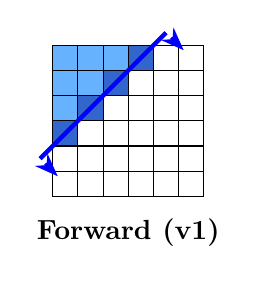
\begin{tikzpicture}[scale=0.32]
    % Grid dimensions
    \def\gridsize{6}

    % Draw forward pass grid (6x6)
    % Index from top-left (0,0) to bottom-right (5,5)
    % Antidiagonal index = i+j (0 to 10)
    % Let's show antidiagonal 3 (B = blue line)
    \def\diagindex{3}

    \foreach \i in {0,...,5} {
        \foreach \j in {0,...,5} {
            \pgfmathtruncatemacro{\diag}{\i + \j}

            % Determine color based on position relative to wavefront
            \ifnum\diag<\diagindex
                % Already processed
                \def\cellcolor{LightBlue}
            \else\ifnum\diag=\diagindex
                % Currently processing (active wavefront)
                \def\cellcolor{DarkBlue}
            \else
                % Not yet processed
                \def\cellcolor{white}
            \fi\fi

            % Draw cell
            \fill[\cellcolor] (\j, -\i) rectangle +(1, -1);
            \draw[black, thin] (\j, -\i) rectangle +(1, -1);
        }
    }

    % Draw diagonal line on wavefront extending past grid
    \draw[blue, ultra thick] (\diagindex+1.5, 0.5) -- (-0.5, -\diagindex-1.5);

    % Arrows at ends of line, offset perpendicular to avoid overlap, pointing bottom-right
    \draw[-{Stealth[scale=1.0]}, very thick, blue] (4.7, 0.3) -- (5.2, -0.2);
    \draw[-{Stealth[scale=1.0]}, very thick, blue] (-0.3, -4.7) -- (0.2, -5.2);

    % Label
    \node[anchor=north] at (3, -6.5) {\textbf{Forward (v1)}};
\end{tikzpicture}

\hspace{1cm}

% Backward Pass Diagram
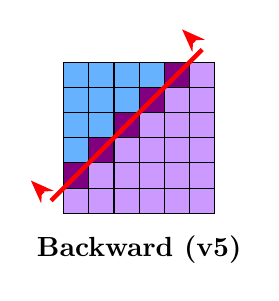
\begin{tikzpicture}[scale=0.32]
    % Grid dimensions
    \def\gridsize{6}

    % Draw backward pass grid (6x6)
    % Wavefront moves from bottom-right to top-left
    % Antidiagonal index = i+j, decreasing from 10 to 0
    % Let's show antidiagonal 4, shifted slightly off-diagonal
    \def\diagindex{4}

    \foreach \i in {0,...,5} {
        \foreach \j in {0,...,5} {
            \pgfmathtruncatemacro{\diag}{\i + \j}

            % Determine color based on position relative to wavefront (reversed)
            \ifnum\diag>\diagindex
                % Already processed by backward
                \def\cellcolor{LightPurple}
            \else\ifnum\diag=\diagindex
                % Currently processing (active wavefront)
                \def\cellcolor{Purple}
            \else
                % Not yet processed by backward (forward values available)
                \def\cellcolor{LightBlue}
            \fi\fi

            % Draw cell
            \fill[\cellcolor] (\j, -\i) rectangle +(1, -1);
            \draw[black, thin] (\j, -\i) rectangle +(1, -1);
        }
    }

    % Draw diagonal line on wavefront through centers of active cells
    \draw[red, ultra thick] (5.5, 0.5) -- (-0.5, -5.5);

    % Arrows at ends of line, offset perpendicular to avoid overlap, pointing top-left
    \draw[-{Stealth[scale=1.0]}, very thick, red] (5.2, 0.8) -- (4.7, 1.3);
    \draw[-{Stealth[scale=1.0]}, very thick, red] (-0.8, -5.2) -- (-1.3, -4.7);

    % Label
    \node[anchor=north] at (3, -6.5) {\textbf{Backward (v5)}};
\end{tikzpicture}

\end{document}
